%!TEX root = ../report.tex

\begin{document}
\chapter{Introduction}

Assessing the knowledge of students is one of the most important phases of the learning process \cite{Mohler2011}. Different forms of assessments that exist today include multiple choice questions, fill-in-the-blanks, essay questions, and short answer questions. Prior works have shown that multiple choice questions and fill-in-the-blanks fail to capture the vital aspects of the acquired knowledge such as reasoning and self-explanation \cite{Wang2008}. In contrast, questions which require the students to construct responses in natural language have been found to be more effective in assessing their grasp on the subject matter \cite{Roy2016a}. Essay questions and short answer questions belong to this category. This work is more concerned about short answer questions where students construct answers in natural language. According to Burrows et al. \cite{Burrows2015}, short answer questions are characterized by the following aspects:

\begin{itemize}
	
	\item "the question must require a response that recalls external knowledge instead of requiring the answer to be recognized from within the question
	
	\item the question must require a response given in natural language
	
	\item the answer length should be roughly between one phrase and one paragraph
	
	\item the assessment of the responses should focus on the content instead of writing style
	
	\item the level of openness in open-ended versus close-ended responses should be restricted with an objective question design."
	
\end{itemize}

Limited availability of teachers, online learning platforms, and individual or group study sessions done outside classrooms necessitated quick and efficient assessment of free text responses \cite{Mohler2011}. In addition, almost 30\% of the teachers' time is spent on grading the assessments \cite{mason2002}. Computer assisted assessment / automatic grading evolved as a solution to this problem and a lot of research has been done on automating the grading of essay \cite{Higgins2004} and short answer responses \cite{Leacock2003, Pulman2005, Mohler2009}. Assessing the students' responses in time and giving faster feedbacks enables the students to realize the mistakes and learn from them or even appear for re-examination without wasting one semester.

Automatic short answer grading essentially deals with using computational methods to compute the grades for students' answers, thus helping the students in getting their feedbacks as soon as possible by heavily reducing the assessing time. Many automated approaches have been proposed in the past for grading short answer questions. Most of these methods include professors penning down the keywords expected in students' answers for every question or handcrafting the patterns and templates against which students' answers are matched to compute the final score. Though these methods managed to perform with reasonable accuracy, non-generalizability is one of the biggest drawbacks. Features such as keywords and pattern templates are very specific to the questions, and the same features cannot be used for new questions and different domains. Thus, a need for a generalized way of extracting features which would solve the problem of grading the answers in new questions and different domains arose and machine learning was considered as a possible solution. Natural language processing and machine learning techniques are used to extract the features from students' answers which are then used to train a model to compute the grades. Machine learning approaches could save the professors' time and effort in finding the best pattern templates and keywords to look for in students' answers.

%These methods compare how similar the students' answers are to the one provided by the teacher or professor and assign a grade proportional to the magnitude of similarity \cite{Mohler2011}. Different approaches of computing these similarity measures include handcrafted pattern matching, automatic pattern matching, lexical similarity (how particular words effect other words), semantic similarity (deals with the meaning of sentences), and entailments (whether one sentence leads to another without any contradiction).

\vspace{3mm}
\begin{figure}[h!]
	\centering
	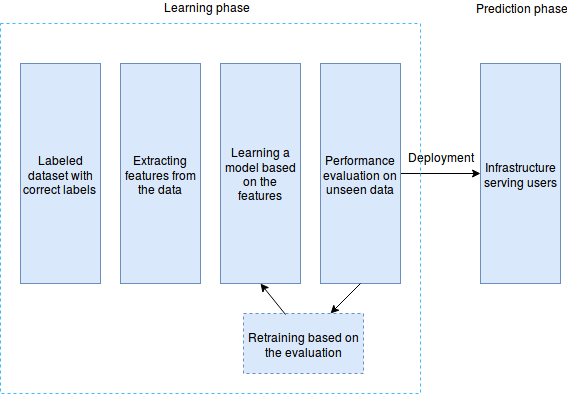
\includegraphics[scale=0.6]{images/simpler_model_1}
	\caption{Workflow of automatic short answer grading \cite{Burrows2015}.}
	\label{auto_workflow}
\end{figure}


Fig \ref{auto_workflow} shows a general workflow of automatic short answer grading as a pipeline. After creating a dataset of all the students' answers and model answers written by the teachers, useful features are extracted from the answers using natural language processing techniques. A model is developed based on these features to calculate the scores and deployed for use. Such a model learns only once from the available set of labeled data and there is no feedback mechanism to fine-tune the parameters based on the wrong predictions after the deployment.


This work proposes an approach where a generic scoring model tries to learn this task of measuring the correctness of each answer continuously with a human in the loop. During the learning stage, the system selects the best samples for the human to grade which would eventually contribute to its knowledge base. Thus, it tries to reduce the human effort of going through all the answers while improving it's understanding of the problem on a cyclical and iterative basis. \\

\begin{figure}[h!]
	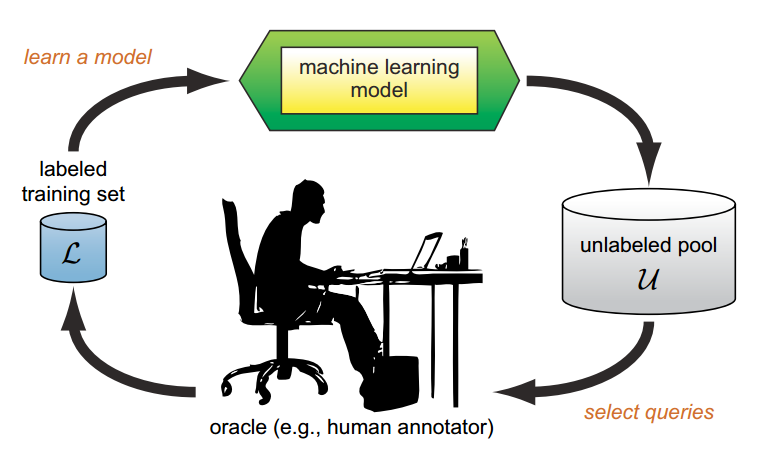
\includegraphics[width=\textwidth]{images/active_learning}
	\caption{Workflow of active learning. Image from \cite{Settles2010}.}
	\label{ac_workflow}
\end{figure}

Active learning seems to be the best choice for this task as it actively queries the human for grades of the samples it is most uncertain of. Fig \ref{ac_workflow} illustrates a typical workflow of active learning. According to Settles \cite{Settles2010}, "it is a subfield of machine learning which works under the hypothesis that if the learning algorithm is allowed to choose the data from which it learns it will perform better with less labeled data and training". Such a model queries a user / human expert for the labels of certain data samples in such a way that it can learn to produce the desired outputs with higher accuracy. By actively selecting the data samples to label, it reduces a considerable amount of labeled training samples, thus, alleviating the problem of insufficient labeled data which is prevalent in supervised learning approaches where a large number of graded answers are used for learning a model. In addition, it would be a solution to deal with the diversity in answers as there is generally no single best response for an open-ended question.

%\section{Motivation}
%
%Limited availability of teachers, online learning platforms, and individual or group study sessions done outside classrooms necessitated quick and efficient assessment of free text responses \cite{Mohler2011}. In addition, almost 30\% of the teachers' time is spent on grading the assessments \cite{mason2002}. Computer assisted assessment / automatic grading evolved as a solution to this problem and a lot of research has been done on automating the grading of essay \cite{Higgins2004} and short answer responses \cite{Leacock2003, Pulman2005, Mohler2009}. Assessing the students' responses in time and giving faster feedbacks enables the students to realize the mistakes and learn from them or even appear for re-examination without wasting one semester. Machine learning approaches could save the professors' time and effort in finding the best pattern templates and keywords to look for in students' answers. The focus of this work would be on improving the existing solutions to grade short answer questions.

\section{Challenges and Difficulties}

The conventional methods in automatic short answer grading belong to a learning paradigm called supervised learning where the right grade for every student answer in the training phase is available. Though these approaches were able to produce decent results, they suffer from many shortcomings such as;

\begin{itemize}
	
	\item lack of sufficient amount of labeled training data in the domain to learn the models. Reasons include annotation cost, privacy, availability, and the quality of the correct answers.
	
	\item the failure to capture the different wordings/phrasing of the students while trying to answer the short answer questions. It is obvious that anticipating all different ways of answering his questions is practically impossible for the professor. 
		
	\item inability to capture consistent patterns of misunderstandings among students. Ability to recognize such patterns would enable the automated systems to provide useful feedback to students as to why there was a reduction in marks awarded.
	
	\item accounting for small deviations in the answers which might affect the whole meaning of the sentence (for ex. in mathematical terms, though each and every word of the student's answer align with that of the professor, a small negation or inverse operation would change the whole meaning).
	
	\item finding a way to understand the underlying concept of various students' answers and bagging the similar ones (or the right and wrong ones separately) is also a very tedious task. 
	
	\item being a passive learner, these models learn the rules once and apply them on new input answers. Thus, it would be very difficult to achieve robustness when applied to new data over time. \\
	
\end{itemize}

\section{Problem Statement}

It is common in the task of short answer grading that obtaining the correct grade for all different types of student answers is time-consuming and subjective to the grader in nature. In addition, it costs more to have a large amount of dataset (questions, answers, and their grades) to train complex models on them. Thus, a mechanism which can learn on a small amount of graded answers obtained through a query strategy and can produce results on the remaining ungraded answers is more appropriate to this task. In contrast to supervised learning, active learning achieves comparable results with less amount of data. Active learning is an algorithm which chooses a small amount of data which is more efficient and more informative to the learning process. Short answer grading is not a "fit once and apply forever" task as new questions are added every now and then, and the students' answers contain a vast range of lexical diversity. Active learning can be easily fitted on a new dataset as it includes an adaptive mechanism of training the model which takes into account the new set of data in addition to the one on which it learned earlier. Hence, active learning is chosen to be evaluated for our task of short answer grading as it has achieved comparable results with supervised learning techniques with less number of labeled data for training \cite{yang2009effective}. 

This work differs from the approach illustrated in Fig \ref{auto_workflow} by incorporating a feedback mechanism which allows the model to learn continuously based on new labeled input samples. As illustrated in Fig \ref{ac_simple_workflow}, we propose a model which implements active learning for the task of short answer grading.

\vspace{5mm}

\begin{figure}[h]
	\centering
	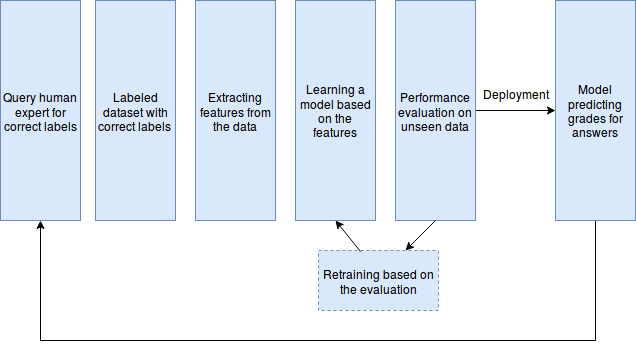
\includegraphics[scale=0.6]{images/simpler_model_ac}
	\caption{Workflow of active learning in automatic short answer grading} %\cite{Burrows2015}.}
	\label{ac_simple_workflow}
\end{figure}

In this research project, various active learning strategies are evaluated as a potential solution to overcome the deficits of automated short answer grading. Thus, issues such as high cost of labeled data, understanding common misconceptions among the students, lexical diversity in answers, and inferior performance are addressed in this work. Various natural language processing techniques such as text preprocessing, semantic similarity, and the best features to be extracted from the answers are experimented for the task of short answer grading. Active learning strategies are evaluated based on aspects such as seed selection, instance sampling, and batch size. The best strategy from each stage is selected for the implementation of the final model. A generic interactive model for assessments in different domains is implemented based on the results of experiments performed using a web-based Graphical User Interface (GUI). All techniques are analyzed on accuracy, reliability, amount of human action(clicks) required, flexibility for different domains, runtime, and user experience. 

\end{document}
